\subsection{Modelo Matemático do Motor CC Série}

Os motores CC série tem como principal característica possuir o enrolamento de campo em série com o enrolamento de armadora, essa configuração resulta em um motor com torque de partida alto, porém, o torque reduz a medida que a velocidade aumenta devido ao aumento da Força Eletromotriz FEM. Por conda desse aumento de FEM os motores CC Séries tem uma regulação de velocidade ruim, quando se aumenta a carga no eixo do motor a velocidade é reduzida que por sua vez reduz a FEM e então o torque aumenta para conseguir atuar na carga.

No entanto, mesmo motores cc série com dimensões reduzidas geram torques altos com baixo consumo de corrente. Visando melhorar seu desempenho, é possível projetar controladores de malha fechada capazes de tornar esses motores mais eficientes na questão da regulação de sua velocidade.

A Figura \ref{fig:image_01} mostra uma diagrama da configuração do motor CC Série, em que o enrolamento de campo está conectado em série com o enrolamento de armadura, dessa forma, a  corrente de campo é igual a corrente de armadura $ i = i_c = i_a$.


\begin{figure}[h]
	\centering
	\caption{Motor CC Série.}
	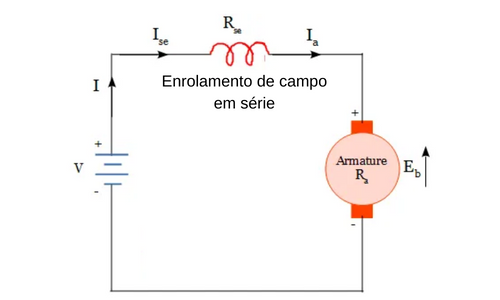
\includegraphics[width=0.6\textwidth]{Capitulos/4_desenvolvimento/4_figuras/esquema_motorcc.png}
	\caption*{Fonte $-$ colocar fonte aqui.}
	\label{fig:image_01}
\end{figure}

Na Figura \ref{fig:image_02}, mostra o diagrama eletromecânico do do Motor CC Série, nele podemos observar que os componentes elétricos estão todos em série, em que o enrolamento de campo possui uma parte resistiva e outra indutiva, assim como o enrolamento de armadura, já a parte mecânica possui uma velocidade angular dada por $\dot{\theta}$, torque eletromagnético do motor dado por $T_e$ e torque da Carga $T_c$.

\begin{figure}[h]
	\centering
	\caption{Diagrama Elétrico/Mecânico Motor CC Série.}
	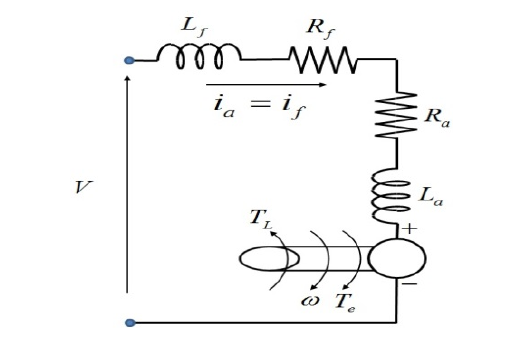
\includegraphics[width=0.6\textwidth]{Capitulos/4_desenvolvimento/4_figuras/diagrama_motorcc.png}
	\caption*{Fonte $-$ colocar fonte aqui.}
	\label{fig:image_02}
\end{figure}



%%%%%%%%%%%%%%%%%%%%%%%%%% Modelagem da Parte Mecânica do Motor CC Série %%%%%%%%%%%%%%%%%%%%%%%%%%
\noindent \textbf{Modelagem da Parte Mecânica do Motor CC Série}

Primeiramente a parte mecânica do motor será modelada, um motor cc série é composto por uma parte rotativa "armadura", de forma que, essa parte, gera um momento de inércia do eixo do motor $J$ e um fator de amortecimento viscoso $b$, além disso, o eixo possui uma velocidade angular $\dot{\theta}$.

Assim, a equação que descreve o modelo mecânico do motor CC Série e dados, por:

\begin{align}
	J\ddot{\theta}(t) &= T_e(t) - b\dot{\theta}(t) - T_c(t) \label{eq4:eq1} \\
	T_e(t) &= J\ddot{\theta}(t) + b\dot{\theta}(t) + T_c(t) \label{eq4:eq2}
\end{align}


Onde:
\begin{itemize}
	\item $T_e$: Torque Eletromagnético produzido pelo Motor;
	\item $J$: Momento de Inércia do Eixo do Motor;
	\item $\ddot{\theta}$: Aceleração Angular do Eixo do Motor;
	\item $\dot{\theta}$: Velocidade Angular do Eixo do Motor;
	\item $b$: Fator de Amortecimento Viscoso;
	\item $T_c$: Torque de Carga.
\end{itemize}

Tanto a Força Eletromotriz $E_A(t)$ quanto o Torque Eletromagnético $T_e(t)$ dependem do fluxo magnético do entreferro $\Phi$, assim, temos as seguintes equações:

\begin{align}
	E_a(t) &= \dot{\theta}(t) \Phi{(i)} \label{eq4:eq3}\\
	T_e(t) &= i(t) \Phi{(i)}			\label{eq4:eq4}
\end{align}

O Fluxo magnético depende da corrente $i(t)$, assim, a equação $(1)$ é não-linear. Além disso, podemos aproximar o fluxo por uma relação linear $K_0$ quando se despreza a saturação magnética.

\begin{align}
	\Phi(i) &= K_0 i(t) \label{eq4:eq5}
\end{align}

A constante $K_0$ é a indutância mútua entre a armadura e o enrolamento de campo.

Agora podemos encontrar o modelo não-linear da parte mecânica do Motor CC Série, substituindo $(5)$ em $(4)$, temos:

\begin{align}
	T_e(t) &= i(t) K_0 i(t) \label{eq4:eq6}\\
	T_e(t) &= K_0 i^2(t) 	\label{eq4:eq7}
\end{align}

Substituindo \ref{eq4:eq2} em \ref{eq4:eq7}, encontramos a modelo da parte mecânica do motor.


\begin{align}
	K_0 i^2(t) &= J\ddot{\theta}(t) + b\dot{\theta}(t) + T_c(t) \label{eq4:eq8}
\end{align}

%%%%%%%%%%%%%%%%%%%%%%%%%% Modelagem da Parte Elétrica do Motor CC Série %%%%%%%%%%%%%%%%%%%%%%%%%%
\noindent \textbf{Modelagem da Parte Elétrica do Motor CC Série}

Para a parte elétrica, vamos usar a lei de Kirchhoff das tensões, como foi dito o motor é um motor CC série, assim, $i_a = i_f$, aplicando Kirchhoff para modelar o sistema elétrico, temos:


\begin{align}
	V(t) &= (R_a + R_f)i(t)+ (L_a + L_f)\frac{d}{dt}i(t) + E_a \label{eq4:eq9}
\end{align}

Onde:

\begin{itemize}
	\item $V$: Tensão da Fonte;
	\item $R_a$: Resistência da Armadura;
	\item $R_f$: Resistência de Campo;
	\item $i_a$: Corrente da Armadura;
	\item $i_f$: Corrente de Campo;
	\item $E_A$: Tensão Contro Eletromotriz Gerada pela Armadura;
	\item $L_a$: Impedância da Armadura;
	\item $L_f$: Impedância de Campo.
\end{itemize}

Como temos os componentes elétricos em série, podemos obter uma resistência total assim como uma indutância:

\begin{align}
	R &= R_a + R_f          \label{eq4:eq10}\\        
	L &= L_a + L_f          \label{eq4:eq11}
\end{align}


\begin{align}
	V(t) &= Ri(t)+ L\frac{d}{dt}i(t) + E_a \label{eq4:eq12}
\end{align}

Substituindo \ref{eq4:eq5} em \ref{eq4:eq3},

\begin{align}
	E_a(t) &= \dot{\theta}(t)K_0 i(t) \label{eq4:eq13}
\end{align}

Agora podemos encontrar a equação de movimento da parte elétrica do sistema ao substituir \ref{eq4:eq13} em \ref{eq4:eq12}:

\begin{align}
	V(t) &= Ri(t)+ L\frac{d}{dt}i(t) + \dot{\theta}(t)K_0 i(t) \label{eq4:eq14}
\end{align}

Equações do Modelo do Motor CC Série.

\begin{align}
	V(t) &= Ri(t)+ L\frac{d}{dt}i(t) + \dot{\theta}(t)K_0 i(t) \label{eq4:eq15}\\
	K_0 i^2(t) &= J\ddot{\theta}(t) + b\dot{\theta}(t) + T_c(t) \label{eq4:eq16}
\end{align}



\subsection{ Modelo Matemático do Aeropêndulo}




\subsection{Junção dos dois Modelos}